%Modified from a template provided by Jennifer Pan, August 2011

\documentclass[10pt,letter]{article}
	% basic article document class
	% use percent signs to make comments to yourself -- they will not show up.
\usepackage{pdfsync}
\usepackage{amsmath}
\usepackage{amssymb}
\usepackage{amsthm}
	% packages that allow mathematical formatting

\usepackage{graphicx}
	% package that allows you to include graphics
\graphicspath{ {./images/} }

\usepackage{setspace}
	% package that allows you to change spacing

\onehalfspacing
	% text become 1.5 spaced

\usepackage{fullpage}
% package that specifies normal margins

\usepackage[parfill]{parskip}

\newtheorem*{thm}{Theorem}
\newtheorem{nthm}{Theorem}
\newtheorem{lem}{Lemma}

\begin{document}
	% line of code telling latex that your document is beginning

\title{Problem Set 3: Checkpoint}

\author{Richard Davis}

% \date{Friday April 10, 2015}
	% Note: when you omit this command, the current date is automatically included
 
\maketitle 
	% tells latex to follow your header (e.g., title, author) commands.


\section*{Checkpoint Question: Love, Love Me Do}
This question explores what happens when you interchange the order of quantifiers in a first-order logic statement. Consider the following two statements in first-order logic:
\begin{equation} \label{chk:a}
\exists x \in P .\ \forall y \in P .\ Loves(x, y)
\end{equation}
\begin{equation} \label{chk:b}
\forall y \in P .\ \exists x \in P .\ Loves(x, y)
\end{equation}
\paragraph{i)} Translate these two statements into English.

Statement \ref{chk:a} can be translated into English as ``there is some person that loves everybody.'' Statement \ref{chk:b} can be translated as ``everybody is loved by somebody.''
\paragraph{ii)} Prove that these statements are not equivalent to one another. To do so, find a group of people $P$ where one of these statements is true and the other is false.

In figure \ref{fig:chk_ii} below we see two groups of people A and B. If two people are connected by an arrow, this means that the person at the base of the arrow loves the person at the tip of the arrow. The person at the bottom-left in group A loves everybody, but none of the other people love anyone. In this group, both statement \ref{chk:a} and statement \ref{chk:b} are true. However, in group B we see that everybody is loved by somebody, but there is no person who loves everyone. In this group, statement \ref{chk:b} is true but statement \ref{chk:a} is false.

\begin{figure}[h]
    \centering
    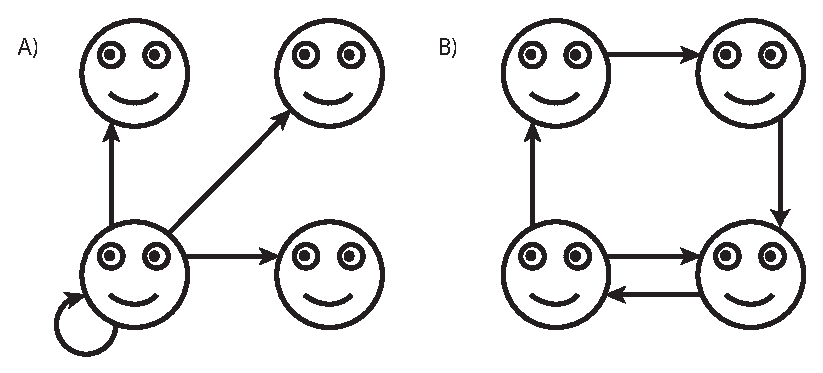
\includegraphics[width=0.7\textwidth]{hw3_checkpoint_ii.eps}
    \caption{Somebody loves everybody (a) and everybody loves somebody (b)}
    \label{fig:chk_ii}
\end{figure}

\pagebreak

\paragraph{iii)} One of these statements implies the other. Determine which statement implies the other, then prove it.

\begin{thm}
Statement \ref{chk:a} implies statement \ref{chk:b}. 
\end{thm}

\begin{proof}
By contradiction. Assume for the sake of contradiction that the theorem is false, that \ref{chk:a} is true and statement \ref{chk:b} is false. 

\begin{align} \label{chk:c}
\exists x \in P .\ \forall y \in P .\ Loves(x, y) &\land \neg(\forall y \in P .\ \exists x \in P .\ Loves(x, y))\\
\exists x \in P .\ \forall y \in P .\ Loves(x, y) &\land \exists y \in P .\ \forall x \in P .\ \neg(Loves(x, y))
\end{align}

The left side of the conjunction says ``There is a person who loves everyone.'' The right side says ``There is a person that nobody loves.'' But this is a contradiction; if there is a person who loves everyone (including herself), then there can not be a person that nobody loves. So the theorem that statement \ref{chk:a} implies statement \ref{chk:b} must be true.

\end{proof}

% \begin{proof}
% By contrapositive. 

% \begin{align} \label{chk:d}
% \neg(\forall y \in P .\ \exists x \in P .\ Loves(x, y)) &\rightarrow \neg(\exists x \in P .\ \forall y \in P .\ Loves(x, y))\\
% \exists y \in P .\ \forall x \in P .\ \neg Loves(x, y)) &\rightarrow \forall x \in P .\ \exists y \in P .\ \neg Loves(x, y))\\
% \end{align}

\end{proof}


% \section*{Appendix: Referencing Equations}
% \begin{equation} \label{eq:divbyzero}
%   \frac {1} {0}
% \end{equation}

% This references \ref{eq:divbyzero}.

\end{document}
	% line of code telling latex that your document is ending. If you leave this out, you'll get an error

%%% Local Variables:
%%% mode: latex
%%% TeX-master: t
%%% End:
